\section{Where can Bioinformatics Help?}

\subsection{Databases and Tools for Analysis}

\begin{frame}[c]{Available Databases are Decentralized}
    \scriptsize
    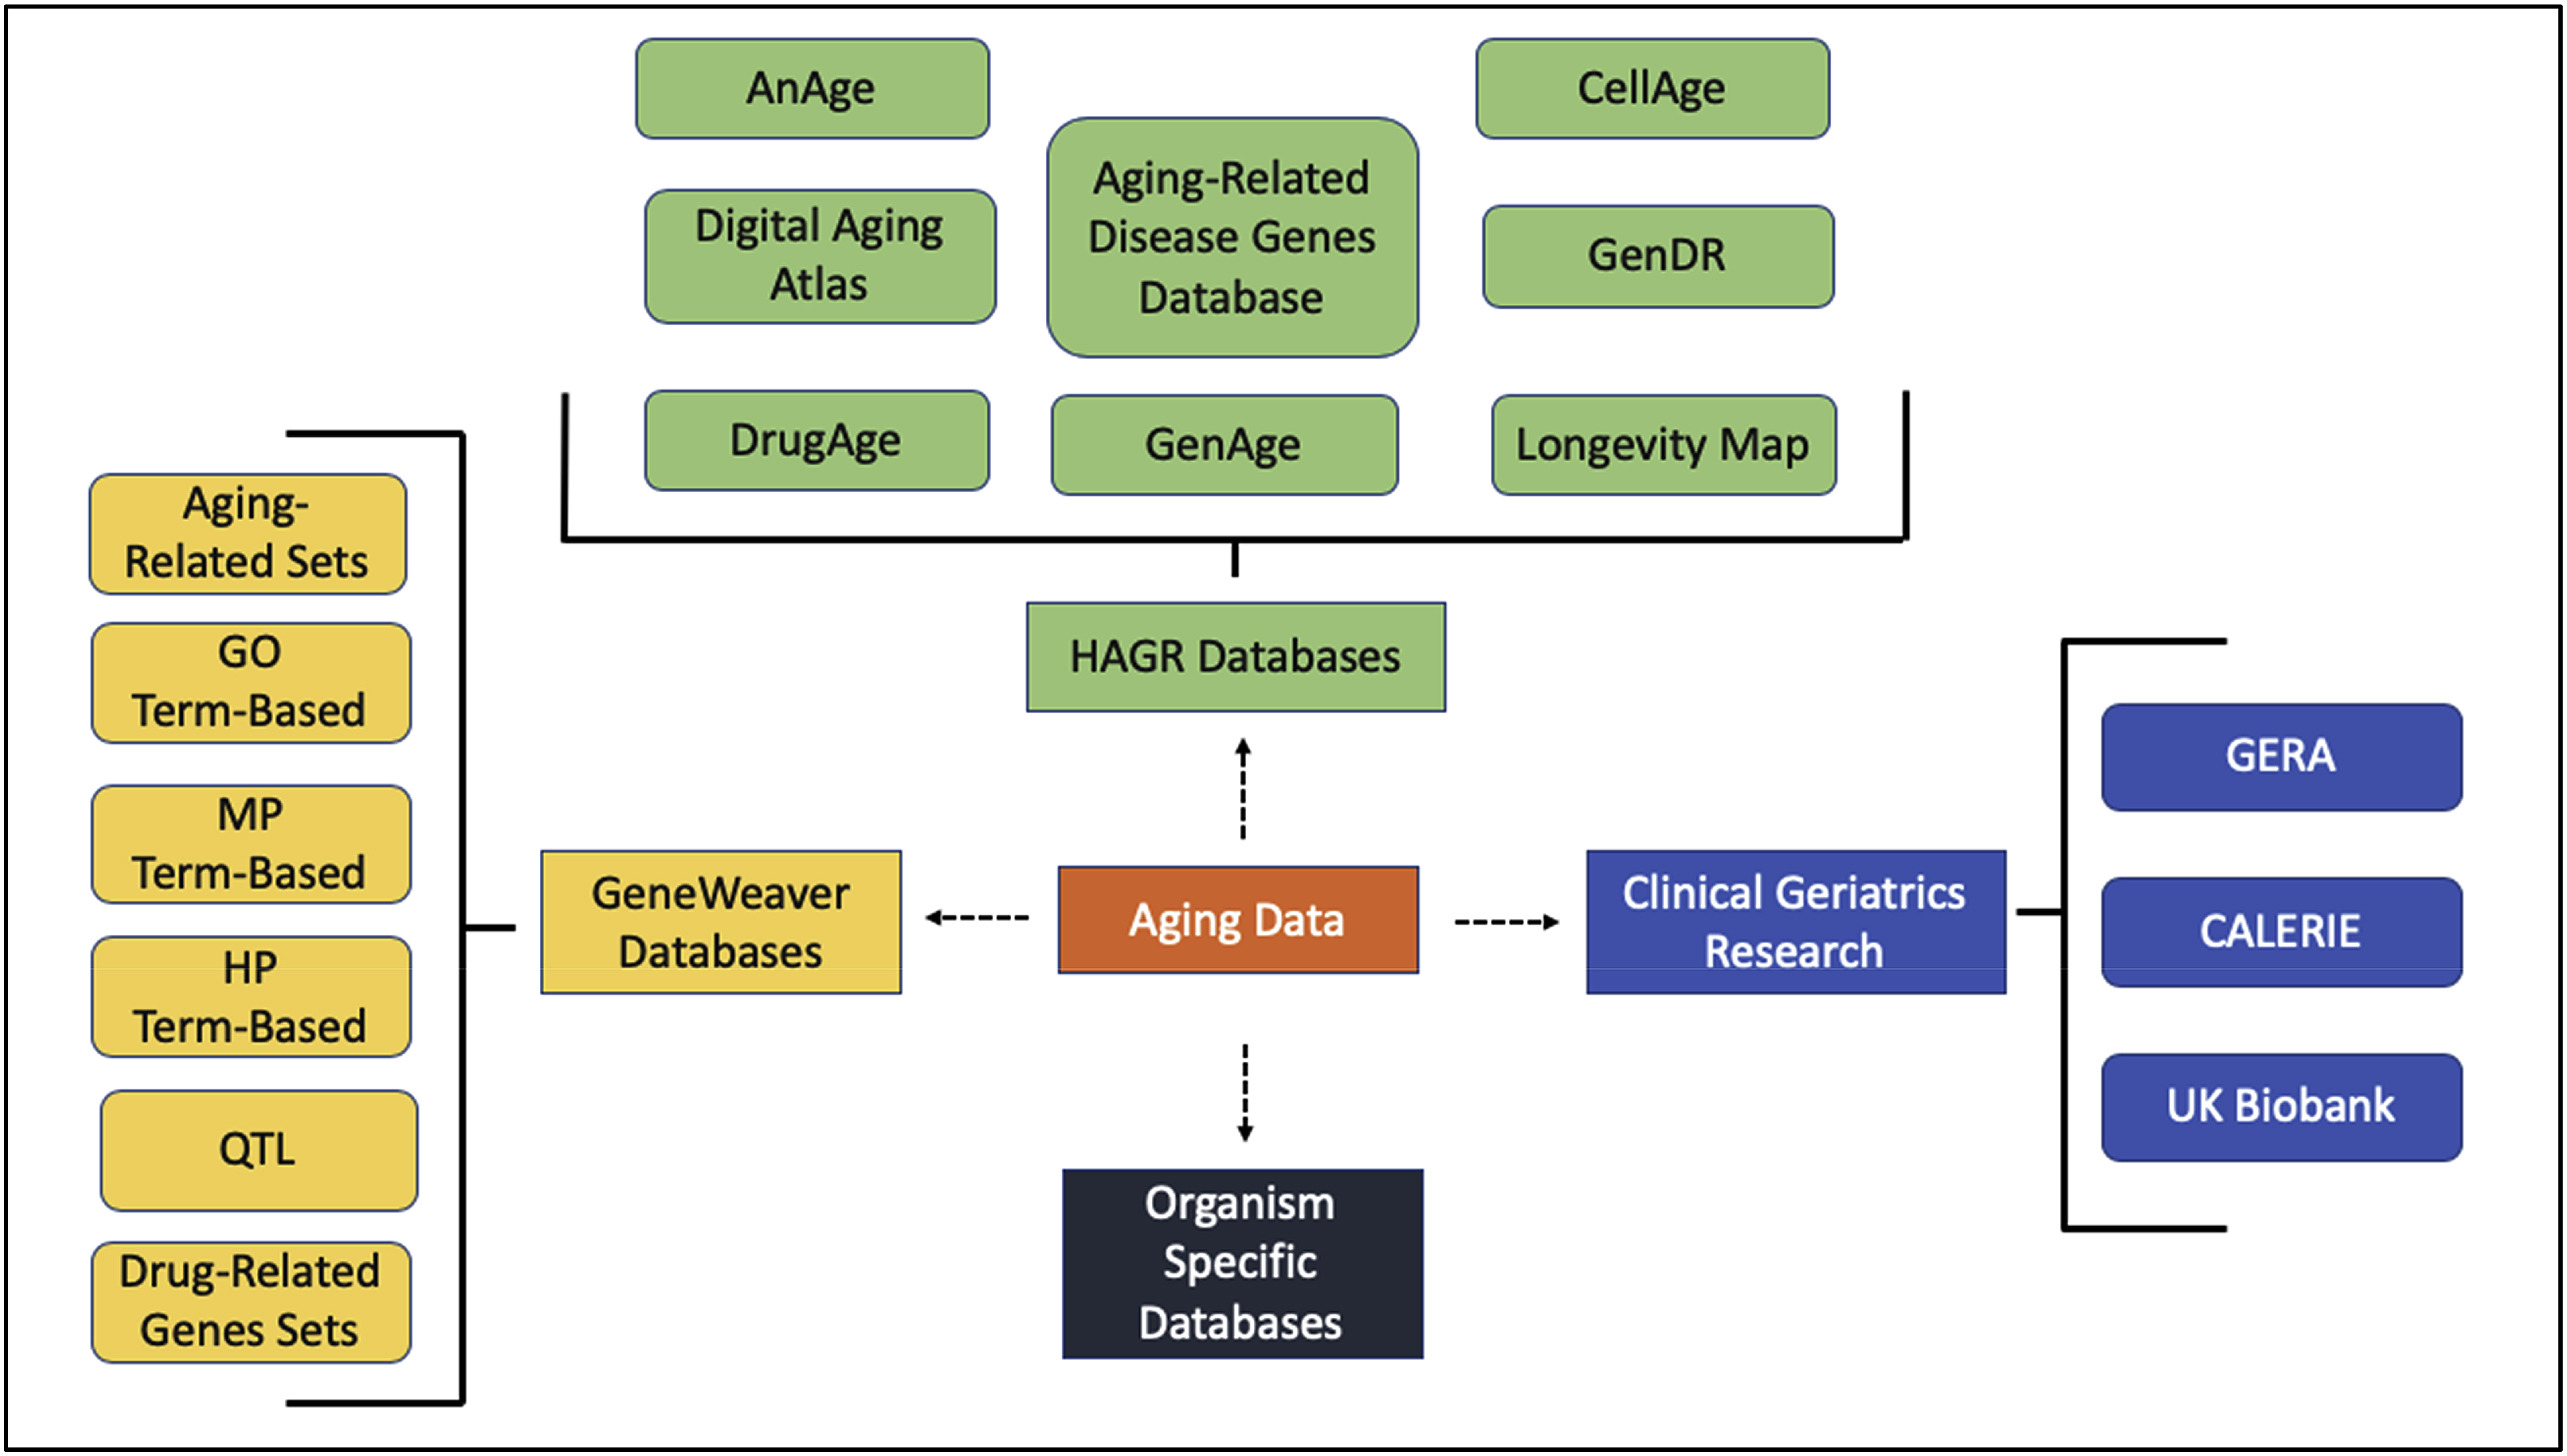
\includegraphics[width=\textwidth]{bioinfo_databases} \\
    Source: \cite{kruempel2019computational}
    \pnote{
        Large number of distributed databases \\
        very difficult to search through multiple \\
        \par
        Next: Computational Tools
    }
\end{frame}


\begin{frame}[c]{Computational Tools}
    \begin{itemize}[<+(1)->]
        \item Prism - statistical analysis and graphing program
        \item Online Application for Survival Analysis (OASIS) - online tool for statistical analysis of lifespan data
        \item R packages: `survival`, `flexsurf`, `survminer` - rapid generation of survival curves and statistical analysis
        \item Machine Learning approaches - gene classification, mortality related biomarker and gene expression profile identification
    \end{itemize}
    \pause
    \scriptsize
    Source: \cite{kruempel2019computational}
    \pnote{
        Exemplary computational tools used \\
        'first iteration' tools \\
        no tools for very sophisticated analysis \\
        Even though we now have some knowledge \\
        \par
        Next: Areas for Improvement
    }
\end{frame}


\subsection{Machine Learning and Aging}

\begin{frame}[c]{Machine Learning for Aging}
    \large
    \begin{itemize}[<+(1)->]
        \item Classifying genes and proteins into aging or non-aging-related \cite{townes2020identifying}
        % \item Classifying genes in model organisms as pro- or anti-longevity \cite{townes2020identifying}
        \item Identification of improved biomarkers for aging in humans \cite{putin2016deep} %, \cite{nakamura2007method}
        \item Establishing aging- and mortality-related gene expression profiles \cite{kerber2009gene}
        \item Much more ...
    \end{itemize}
    \pnote{
        Found new genes related to aging, were unknown
        \par
        A lot of progress happening recently \\
        But only sporadically, a lot more possible
        \par
        AlphaFold2 basically obliterated the competition \\
        Improving and building upon these methods \\
        \par
        Next: Conclusion
    }
\end{frame}

  % Sergey Ovchinnikov, Gyu Rie Lee, Jue Wang, Qian Cong, Lisa N. Kinch, R. Dustin Schaeffer, Claudia Millán, Hahnbeom Park, Carson Adams, Caleb R. Glassman, Andy DeGiovanni, Jose H. Pereira, Andria V. Rodrigues, Alberdina A. van Dijk, Ana C. Ebrecht, Diederik J. Opperman, Theo Sagmeister, Christoph Buhlheller, Tea Pavkov-Keller, Manoj K. Rathinaswamy, Udit Dalwadi, Calvin K. Yip, John E. Burke, K. Christopher Garcia, Nick V. Grishin, Paul D. Adams, Randy J. Read, David Baker},
  % author={Minkyung Baek, Frank DiMaio, Ivan Anishchenko, Justas Dauparas, Sergey Ovchinnikov, Gyu Rie Lee, Jue Wang, Qian Cong, Lisa N. Kinch, R. Dustin Schaeffer, Claudia Millán, Hahnbeom Park, Carson Adams, Caleb R. Glassman, Andy DeGiovanni, Jose H. Pereira, Andria V. Rodrigues, Alberdina A. van Dijk, Ana C. Ebrecht, Diederik J. Opperman, Theo Sagmeister, Christoph Buhlheller, Tea Pavkov-Keller, Manoj K. Rathinaswamy, Udit Dalwadi, Calvin K. Yip, John E. Burke, K. Christopher Garcia, Nick V. Grishin, Paul D. Adams, Randy J. Read, David Baker},

\subsection{Improving Software for Biology}

\begin{frame}[c]{Protein Folding Competition Results (CASP14, 2020)}
    \scriptsize
    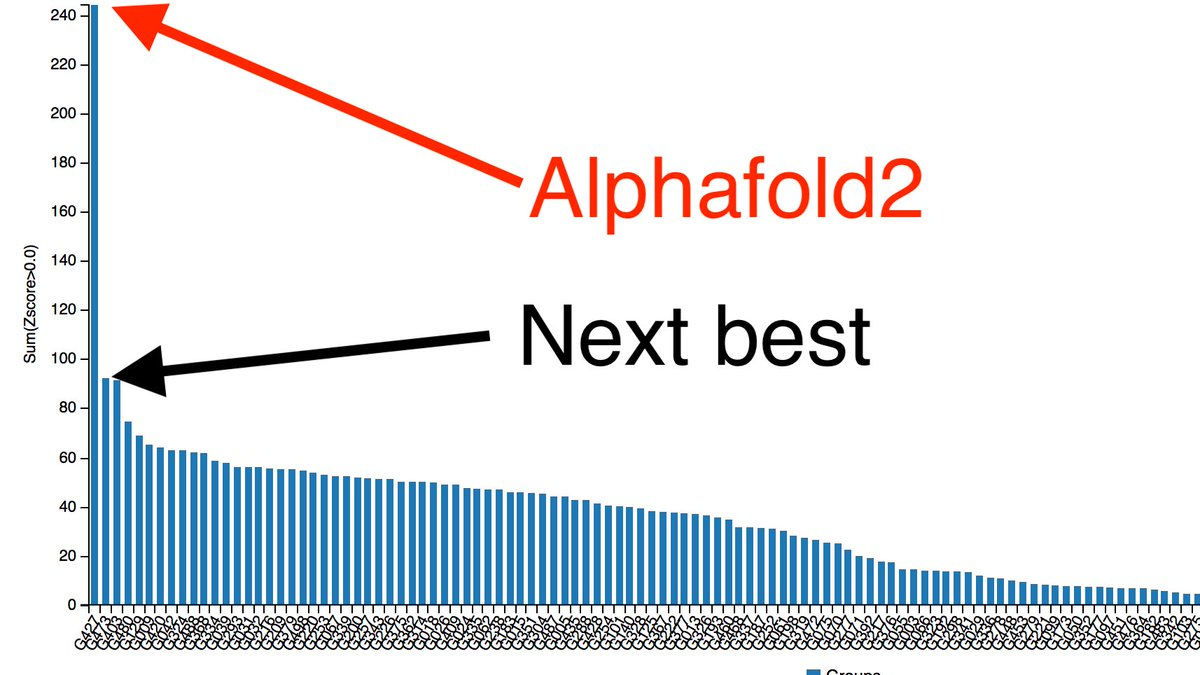
\includegraphics[width=\textwidth]{alphafold_domination}
    Source: \cite{jameswag39:online} \\
    \normalsize
    Recent Breakthrough: AlphaFold2 \cite{jumper2021alphafold} \\
    % \pause
    % \scriptsize
    % (sometime later: RoseTTAFold \cite{baek2021rosetta})
\end{frame}


\begin{frame}[c]{Bioionformatics helping Anti-Aging Research}
    \large
    \begin{itemize}[<+(1)->]
        \item Most software used is not specialized
        \item Providing centralized Database-Access
        \item Maybe: Sophisticated tools for analysis
        \item A lot of basic research still necessary \\(and in progress)
        \item Powerful simulations might be useful
    \end{itemize}
    \pause
    Fundamentally speaking: Provide good Software for Biologists!
\end{frame}


% \begin{frame}[c]{Areas for Improvement}
%     \large
%     \begin{itemize}[<+(1)->]
%         \item Centralized access to Databases - making study data available for further analysis in a {\em centralized} manner
%         \item Increased Biobank usage - collecting biological and clinical data on representative populations
%         \item Sophisticated Tools for Analysis - for the next tier of qualitative analysis 
%         \item Standardization - for easier access and interoperability
%     \end{itemize}
%     \pnote{
%         easier access to data \\
%         more and higher quality data \\
%         awesome tools, but more sophistication possible \\
%         \par
%         Next: Machine Learning
%     }
% \end{frame}


% \begin{frame}[c]{Analysis}
%     \large
%     Large datasets, ever-more data

%     \begin{itemize}[<+(1)->]
%         \item Every medical database getting larger (picture would be great)
%         \item Countries started biobanks (Denmark, UK, ...) (check for source)
%         \item No one attempts analysis: no one has appropriate tools!
%         \item needed: correlating genes with injuries/health problems/allergies over lifetime
%         \item new tools, new bigger better software and comp capacity
%     \end{itemize}
% \end{frame}


% \subsection{Simulation}

% \begin{frame}[c]{Simulation}
%     current Pharmaceutical battle: better simulator (find source with details or picture)
% \end{frame}

% \begin{frame}[c]{Simulation II}
%     AlphaFold2 and others are getting better and better
% \end{frame}

% \begin{frame}[c]{Simulation: Impact}

%     \begin{itemize}[<+(1)->]
%         \item cheaper preliminary analysis
%         \item identification of missing or additional effect pathways
%         \item faster research iterations
%     \end{itemize}
% \end{frame}
